\chapter{后Offer时代}
\newpage
恭喜你获得了Offer,在兴奋之余,希望你明白,在离开美丽的校园之前,你还需要做很多的事情。多打听,多询问,多查阅资料,相信\href{http://bbs.nju.edu.cn/file/S/superphoenix/LSFF.htm}{百合的飞跃攻略}上就已经有足够的信息。本章旨在补充一些信息,希望对即将飞跃重洋的诸位有所帮助。此外,最重要的提示就是\textbf{按照学校给予的Instructions}来有条不紊地展开各种赴美准备工作。
\section{签证准备}
本节向大家提供关于签证准备的一些信息。
\subsection{知道自己的I-20 Number}
一般而言,学校I-20表格都是通过快递寄来的。而一些学校很贴心地在通知快递寄出的邮件中会附上I-20 Number,实际上有了这个Number之后,我们就可以开始下面的步骤而不需要等到I-20寄到。当然保险的做法是收到I-20之后检查上面的信息是否正确。在所有信息无误之后,我们就可以开始准备签证了。根据签证官网给出的\href{http://www.ustraveldocs.com/cn_zh/cn-niv-visaapply.asp}{流程},我们首先需要准备签证所用的照片。一般而言大家去照相馆完成拍摄即可,记得带U盘拿到电子版,因为填写DS-160表格的时候,需要上传照片。\par
\subsection{流程}
\begin{enumerate}
\item 在线填写DS-160表格
\item \href{https://cgifederal.secure.force.com/?language=Chinese\%20(Simplified)\&country=China}{在线}创建账户,确定预约日期与时间。一定记住预约的CGI Reference Number。具体教程\href{http://www.usaqianzheng.com/2013/03/\%E5\%A6\%82\%E4\%BD\%95\%E8\%8E\%B7\%E5\%BE\%97\%E7\%BE\%8E\%E5\%9B\%BD\%E7\%AD\%BE\%E8\%AF\%81\%E7\%9A\%84cgi\%E5\%8F\%B7\%E7\%A0\%81\%EF\%BC\%8Ccgi\%E7\%BC\%96\%E5\%8F\%B7\%E5\%9C\%A8\%E5\%93\%AA\%E9\%87\%8C\%E6\%89\%BE\%EF\%BC\%9Fcgi-reference-number.html}{戳我}。
\item 在线/去中信银行网店 支付签证费用。(目前在线支付,其他银行的网银需要支付额外费用。最近的地点是学校门口的中信ATM机。)
\item 准备预约需要携带的材料和补充材料,安排行程。
\item 面签。
\item 等待中信银行短信/email通知,到网上系统指定的中信银行网点领取自己的护照,记得带身份证和面签预约单。
\end{enumerate}\par

对于需要办理赴加拿大签证的同学,根据加拿大的签证规定,你们不需要面签只需提交材料。具体步骤可以参考\href{http://www.eduwo.com/canprocess/46765.htm}{加拿大签证流程}。

\subsection{面签问题}
我们收录了在赴美面签过程中被面试官问到的一些问题。希望对以后的孩子们有帮助。面签基本上是很轻松的,面试官(VO)也没有问很刁钻的问题。\\
~\\
\textbf{小X回忆}:\\
VO: So which university will you study at?  X: xx Univerisity.\\
VO: (看了一眼I-20上的项目信息)You will study infomation technology, so what's information technology? X: Information technology is about utilizing comptuer science to converte data into valuable information.\\
VO: What's valuable information? X: Valuable information is the usable infomration we get from massive data such as the future customer number, net profit and so on.\\
\textbf{小M回忆}:\\
去哪个学校;学什么。本来在哪个学校;学什么。爸妈的工作是啥;具体是做什么的。你会不会回中国,为什么。\\
\textbf{小G回忆}:\\
Which field are you interested in in computer science? Brief introduction of this field.\\
\textbf{小Y回忆}:\\
VO:你现在在做什? 小Y:我说还没毕业,呆在学校里的。 \\VO吐槽:无法理解为什么这么多中国人去学cs。 小Y:cs很有意思啊!而且很有用啊!\\VO非常有远见地指出:这么多人去学,cs会变得很competitive。 小Y:没错。

\section{机票预订}
本节向大家提供一些机票网址。\par
一般而言,机票购买分为三类:官网购买、其他网站购买(类似qunar.com)、代理购买。
\subsection{官网购买}
官网购买是最放心的一种购买方式,不过可能价格上也会贵一点。笔者在购买机票的过程中,发现在日本过夜转机需要办理过境签并且需要住宿,而全日空官网购买的机票就提供免费住宿而其他网站购买的机票是无法提供的。并且,有的时候官网的价格也会很低。比如笔者就曾在韩亚航空官网买到6k软妹币的往返机票。
\subsection{其他网站}
按照一篇人人日志里面的说法,“一般的国际机票可以提前三个月就关注,有好的就入手,飞前一个半月一定要定下来”,买国际机票和买股票有些类似。个人推荐studentuniverse.com和kayak.com。这两个网站没事可以多刷刷。
\subsection{机票代理}
通过代理购买有好有坏,存在被坑的危险性,所以请大家谨慎购买,没有出票并在官网验证前,不要支付全额费用。
\subsection{Tips}
并不是所有的同学都住在北上广这些地方,所以对于小地方的同学而言,大部分要通过其他方式到到达北上广乘坐国际航班。笔者建议在搜索机票的时候就可以直接搜索所在城市至美国目的地的机票,这样不仅可以从自己家出发坐飞机去上海转机(推荐购买到浦东机场的飞机),而且这样的联票即使在国内航段,也是享受北美航线的行李托运规定的。
\section{体检与疫苗}
不同学校对于体检和疫苗有着不同的要求。有的学校有明确规定,有的学校则没有规定。笔者认为,为了自己今后的安全,做一个体检和必要的疫苗是很有用的。获得出入境体检的健康证后,可以作为以后医疗保险中向保险公司提供的材料,如果在体检中发现了一些健康问题,我们也可以尽量在国内完成治疗以免到美国之后治疗所带来的高昂医疗费用。至于疫苗方面,则根据学校的不同而有所不同,一般学校的Health Center会email你相关信息。如果你想打疫苗,必须先在这里体检,然后办理健康证。\par
\href{http://bbs.nju.edu.cn/file/S/superphoenix/LSFF.htm}{百合的飞跃攻略}有关于在南京办理出国体检和疫苗注射的详细手册,推荐遵照该攻略中的信息进行体检\&疫苗注射,需要更新的是目前营业时间提前到了早上8:00。注意早上不要吃早餐,会影响到身体检查。
\section{住宿}
租房问题相信对于大多数同学来说是非常重要的,一个好的居住环境能够帮助大家更快的融入异国的环境。在国外住宿一般而言有三种方式:学校宿舍、合租/单人租、Homestay。其中Homestay是研究生不太经常的选择,所以这里不赘述了。
\subsection{学校宿舍}
一般而言,学校宿舍提供的环境会比自己在外面租好一些,同时价格上也有着相应的体现。学校住宿好处在于离学校近、相对在外住宿比较安全、能够有同龄的外国舍友。所以如果学校住宿的价格是你可以接受的话,在学校住宿是一个不错的选择。需要提醒的是有的学校对于住宿生有额外的疫苗要求,比如需要注射乙肝疫苗等等。这个需要同学们在打疫苗的时候留心学校的要求。
\subsection{校外租房}
相信大部分的人还是需要在校外租房的,因为一是学校的宿舍有限而又大部分向低年级的学生倾斜,还有一个原因就是自由度更大一些。你能够选择1-2两个觉得不错的朋友一起合租,这样也没有和外国人合租可能会导致的一些尴尬。对于在外租房,需要提醒大家的一是注意安全,另外一个就是deposit。在入住之前,房东一般都要求交给半个月到一个月房租不等的deposit,在居住期间发生了折旧或者损坏会从deposit中扣除。因此如果rp不好遇上了不是很nice的房东,你可能一分钱都要不回来了。\par
关于什么样的房东我觉得还是要自己去看看才会明白,很多房东在收钱之前很nice,但是收钱之后就不一定了,所以之前去的人的评价就很重要。笔者建议是向学长学姐打听而不要太相信网上的评论。比如笔者曾经租的一个house,中介是一对中国夫妇开的,就十分nice,环境也十分好。但是网上只给了3颗星的评价并说房子里面有老鼠什么的,笔者觉得这个就有点扯了。\par
此外在校外居住一定要\textbf{注意安全},贵重的物品要学会放好,不要露富。
\section{档案与户口}
对于要出国的同学,如果户口当初迁到了学校,那么毕业后,需要迁回原籍。关于出国留学人员的档案和户口问题,学校给出的官(mei)方(yong)指导意见可以\href{https://www.evernote.com/shard/s51/sh/c4b48b91-d3e3-44c3-8921-1448b76d3e5f/e7fbecd380cc0a83277316c2949609e5}{戳我}。实际上我们有两种套餐,小编接下来慢慢讲述。
\subsection{生死相连套餐}
所谓生死相连实际上是说户口和你的档案都迁回自己家乡的人才市场。每个地方的收费好像不太一样。这样的好处就是户口和档案在一起,方便管理。此外如果在国外时间超过了当初购买的保管期限,父母亲帮你续交的话会比较方便。如果打算长期在国外居住,不准备回国找工作的话,这样处理是不错的。\par
毕业的时候你会拿到报到证和户口迁移表。报到证和户口迁移表是你办理\textbf{档案户口的重要资料},千万保管好。大约8月初等档案通过学校寄到了人才市场,去人才市场办理手续就可以关于人才市场的操作就不赘述了,因为比较简单。
\subsection{异地分居套餐}
所谓异地分居就是将档案寄送到教育部留学服务中心档案室,而将户口迁回自己家(注意不是人才市场,因为好像没听说过户口可以单独放在人才市场的)。这样做的好处就是,在出国回来后办理学位认证方便一些。因为如果留学后想回国找工作,是需要带档案和在国外的相关材料去留学服务中心办理国外学位认证的(否则你在国内找工作就只能拿本科的学历),所以档案放那边到时候办理认证方便一些。不然需要去人才市场拿出档案后,再去北京办理。\par
但是这样做手续比较繁琐。首先,你需要通过邮寄方式办理\href{https://www.evernote.com/shard/s51/sh/14ca023f-da28-4bb7-9c27-8f7f8da89fdd/6dc819d3c82f8f739dd2d88884105338}{档案管理},交给老师留服开出的调档函。然后,在学校的就业去向信息中,按如下信息填写:
\begin{center}
\begin{tabular}{|l|l|}
\hline
项目 & 信息 \\ \hline
报到证单位信息 & 家乡人才市场的信息 \\
档案接收单位信息 & 留学服务中心的信息\\
户口迁移单位信息 & 家乡人才市场的信息/自己家的户口信息\\ \hline
\end{tabular}
\end{center}\par
关于户口还需要补充,如果迁回原籍,那么无论你户口信息填的是否是当地人才市场,学校迁出的时候只能开出到家乡的人才市场。如果你需要再迁回自己家,和爸妈在一张户口本上,那么需要你带齐相关材料,到人才市场咨询详细过程后办理。

\subsection{小结}
说起来很复杂,下面用图来总结下大致流程。\\
\begin{figure}[htbp]
\centering
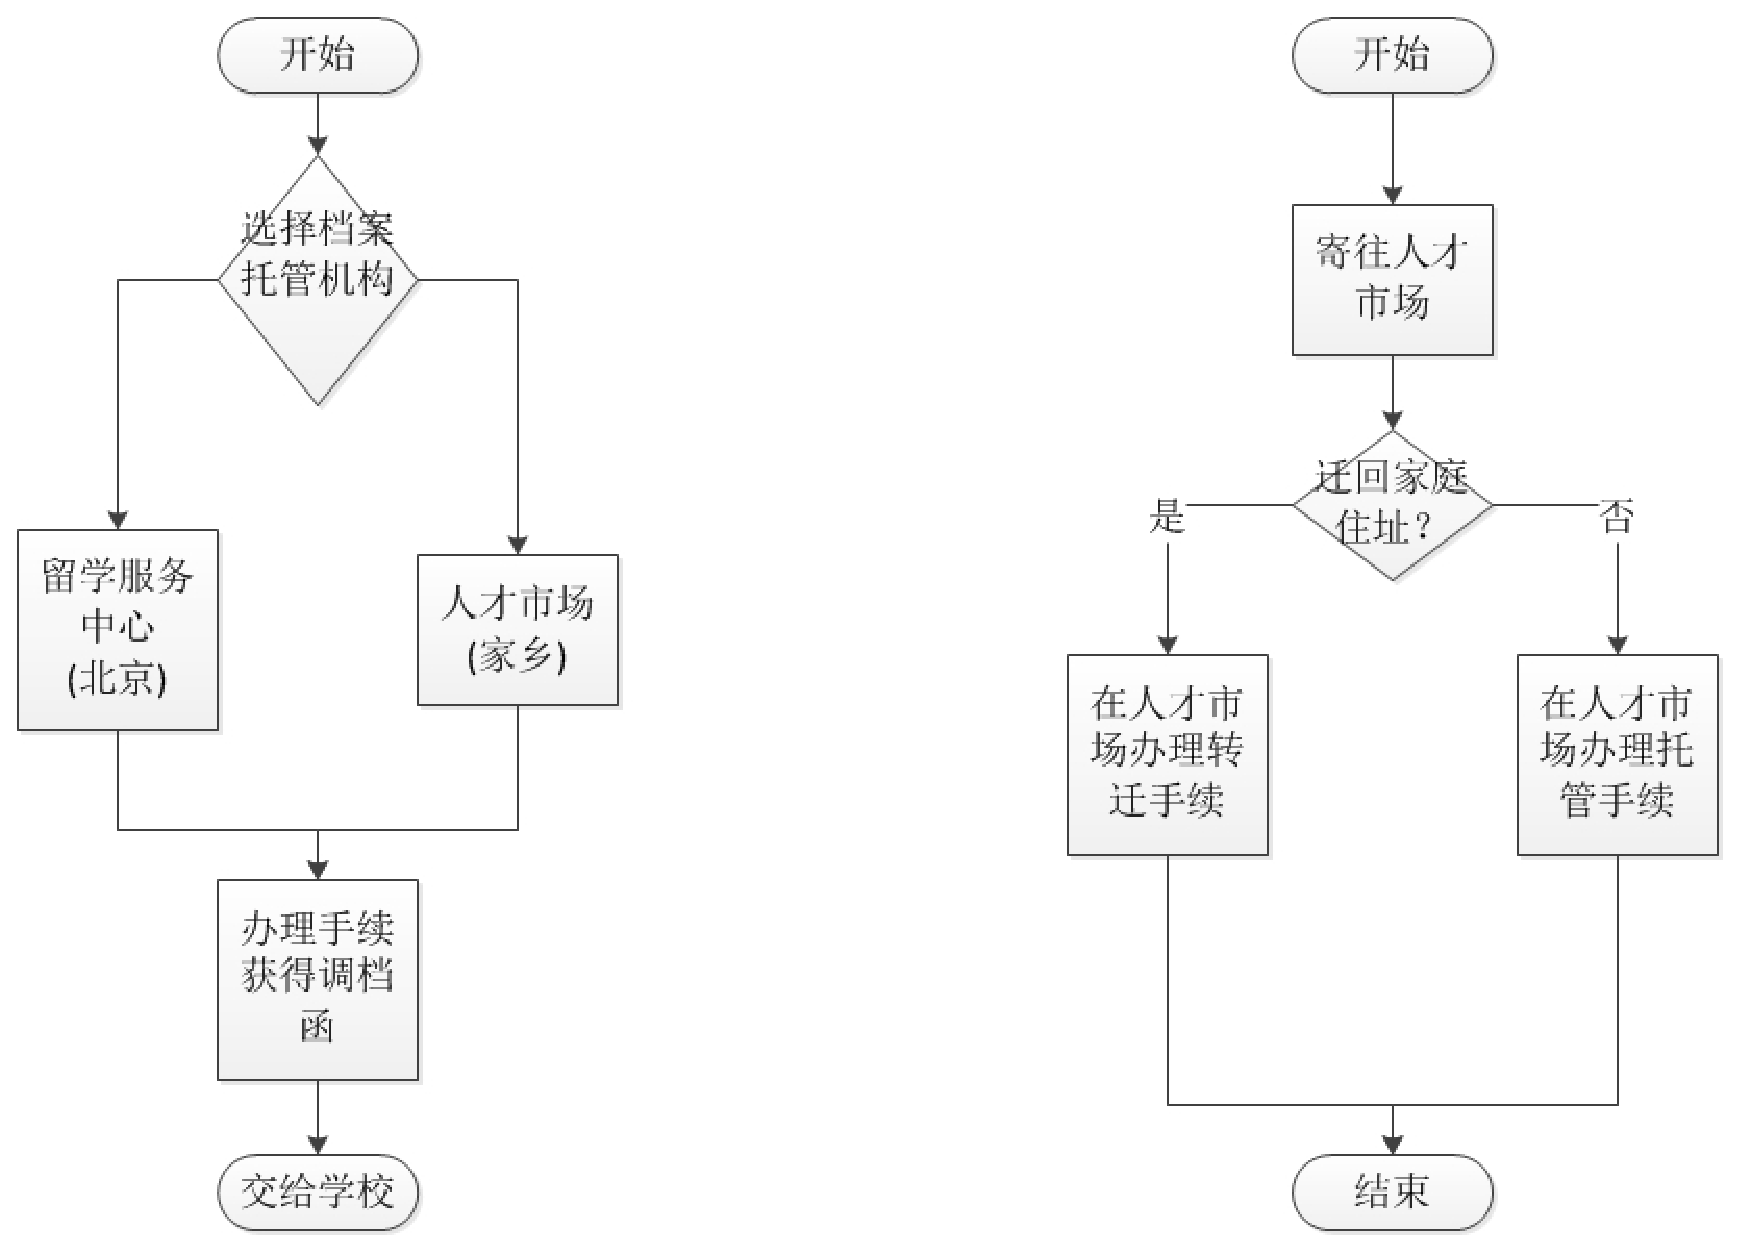
\includegraphics[width=12cm]{4postoffer/hukou.eps}
\end{figure}\par
